\chapter{Исследования характеристик источника тока}

\section{Цель работы}
Исследовать зависимость полной мощности, полезной мощности, мощности потерь, падения напряжения во внешней цепи и КПД источника от силы тока в цепи

\section{Ход работы}

\begin{table}[h]
	\caption{}
	\centering
	\begin{tabular}{|c|c|c|c|c|c|c|c|c|c|c|c|c|c|c|c|}
		\hline
		R, Ом & 100 & 200 & 300 & 400 & 500 & 600 & 700 & 800 & 900 & 1000 \\ \hline
		U, В & 19.2 & 16.9 & 15.0 & 13.2 & 12.0 & 11.1 & 10.3 & 9.5 & 8.8 & 8.1 \\ \hline
		I, А & 1.007 & 2.23 & 3.54 & 4.76 & 5.53 & 6.14 & 6.69 & 7.20 & 7.69 & 8.13    \\ \hline
	\end{tabular}
\end{table}

\begin{figure}[h]
	\centering
	\caption{График зависимости напряжения $U$ от силы тока $I$}
	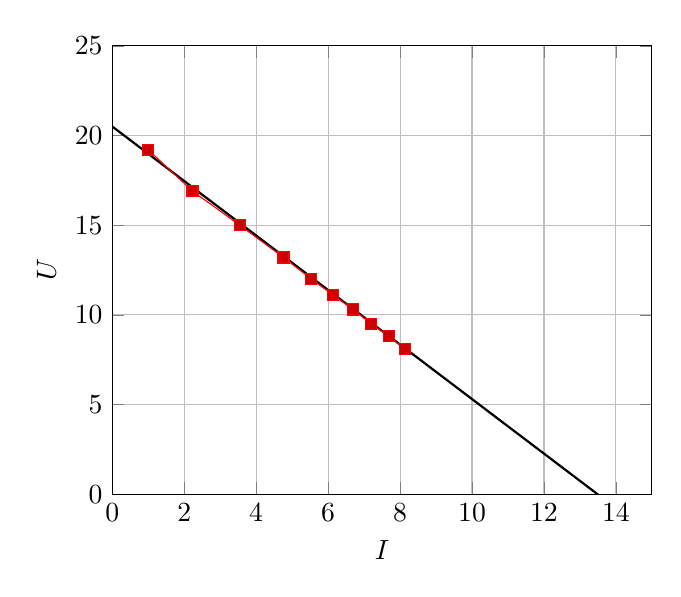
\begin{tikzpicture}
	\begin{axis}[
	xlabel=$I$,
	ylabel=$U$,
	xmin=0, xmax=15,
	ymin=0, ymax=25,
	grid=major
	]
	\addplot [smooth, thick, domain=0:15]{20.5-1.52*x};
	\addplot coordinates {
	(1.00, 19.2)
	(2.23, 16.9)
	(3.54, 15.0)
	(4.76, 13.2)
	(5.53, 12.0)
	(6.14, 11.1)
	(6.69, 10.3)
	(7.20, 9.5)
	(7.69, 8.8)
	(8.13, 8.1)	
	};
	\end{axis}
	\end{tikzpicture}
\end{figure}

Экстраполируя график до пересечения с осями координат, получаем:
\[
\varepsilon = 20.5 \text{ [В]}, I_K = 13.4 \text{ [А]}
\]

Определим внутреннее сопротивление источника $r$
\[
r = \frac{\varepsilon}{I_K} = \frac{20.5}{13.4} = 1.529
\]

Рассчитаем мощности $P$, $P_1$, $P_2$ и КПД $\eta$ для измеренных значений силы тока. Построим график зависимостей этих величин от силы тока.

\[
P = P_1+ P_2, P_1 = \varepsilon \cdot I  - I^2\cdot r, P_2 = I^2 \cdot r
\]

\begin{figure}[h]
	\centering
	\caption{График зависимости мощностей от силы тока $I$}
	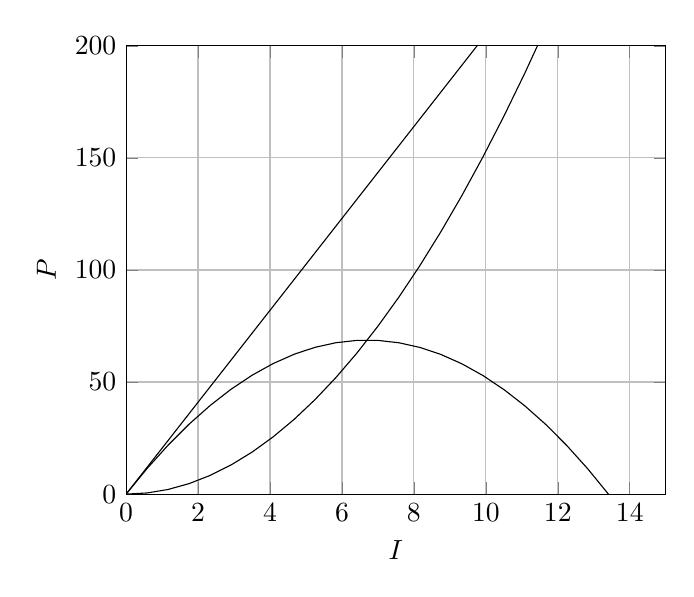
\begin{tikzpicture}
	\begin{axis}[
	xlabel=$I$,
	ylabel=$P$,
	xmin=0, xmax=15,
	ymin=0, ymax=200,
	grid=major
	]
	\addplot [domain=0:14]{20.5 * x};
	\addplot [domain=0:14]{20.5 * x- x * x * 1.529};
	\addplot [domain=0:14]{x * x * 1.529};	
	\end{axis}
	\end{tikzpicture}
\end{figure}

\begin{figure}[h]
	\centering
	\caption{Зависимость КПД источника от силы тока в замкнутой цепи}
	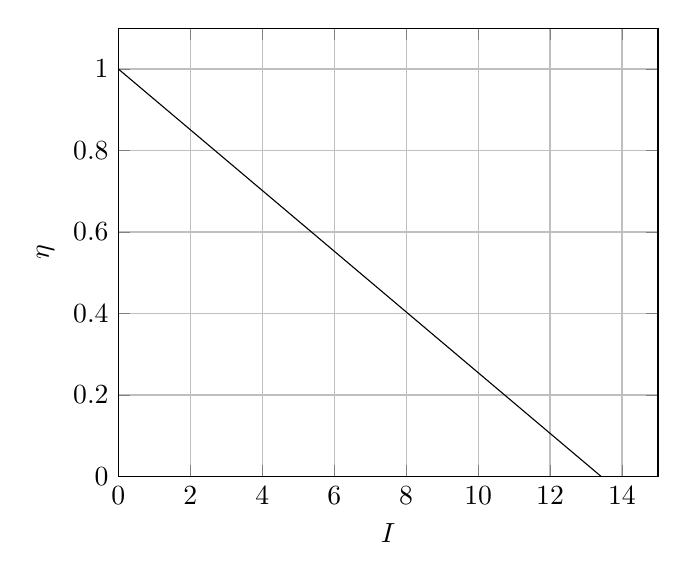
\begin{tikzpicture}
	\begin{axis}[
	xmin=0, xmax=15,
	ymin=0,
	grid=major,
	xlabel=$I$,
	ylabel=$\eta$]
	\addplot [domain=0:20]{1-x*1.49/20};
	\end{axis}
	\end{tikzpicture}
\end{figure}